\documentclass{beamer}

\usetheme{Madrid}
\usepackage[utf8]{inputenc}
\usepackage[T1]{fontenc}
\usepackage{graphicx}

\title{Equity-Aware Ambulance Outpost Siting in Sar{\i}yer}
\author{INDR 486/586 Term Project}
\date{\today}

\begin{document}

\begin{frame}
\titlepage
\end{frame}

\begin{frame}{Problem Motivation}
\begin{itemize}
    \item Emergency response access depends strongly on facility location.
    \item Sar{\i}yer has spatially dispersed neighborhoods and uneven accessibility.
    \item The project asks where ambulance outposts should be located to improve access.
    \item We evaluate both efficiency and equity.
\end{itemize}
\end{frame}

\begin{frame}{Data}
\begin{itemize}
    \item 10 selected demand neighborhoods.
    \item Population is used as demand weight.
    \item 7 candidate public facilities.
    \item Driving distances are represented by a seed distance matrix.
    \item Optional final version can refresh distances using OSRM or openrouteservice.
\end{itemize}
\end{frame}

\begin{frame}{Optimization Model}
\begin{itemize}
    \item Binary variable $y_j$: whether facility $j$ is opened.
    \item Binary variable $x_{ij}$: whether neighborhood $i$ is assigned to facility $j$.
    \item Objective: minimize population-weighted average distance.
    \item Constraint: each demand point assigned to one open facility.
    \item Constraint: at most $P$ facilities can be opened.
\end{itemize}
\end{frame}

\begin{frame}{Equity Metrics}
\begin{itemize}
    \item Maximum assigned distance.
    \item Weighted 90th percentile distance.
    \item Weighted coefficient of variation.
    \item Weighted Gini coefficient.
\end{itemize}
\end{frame}

\begin{frame}{Efficient Frontier}
\centering
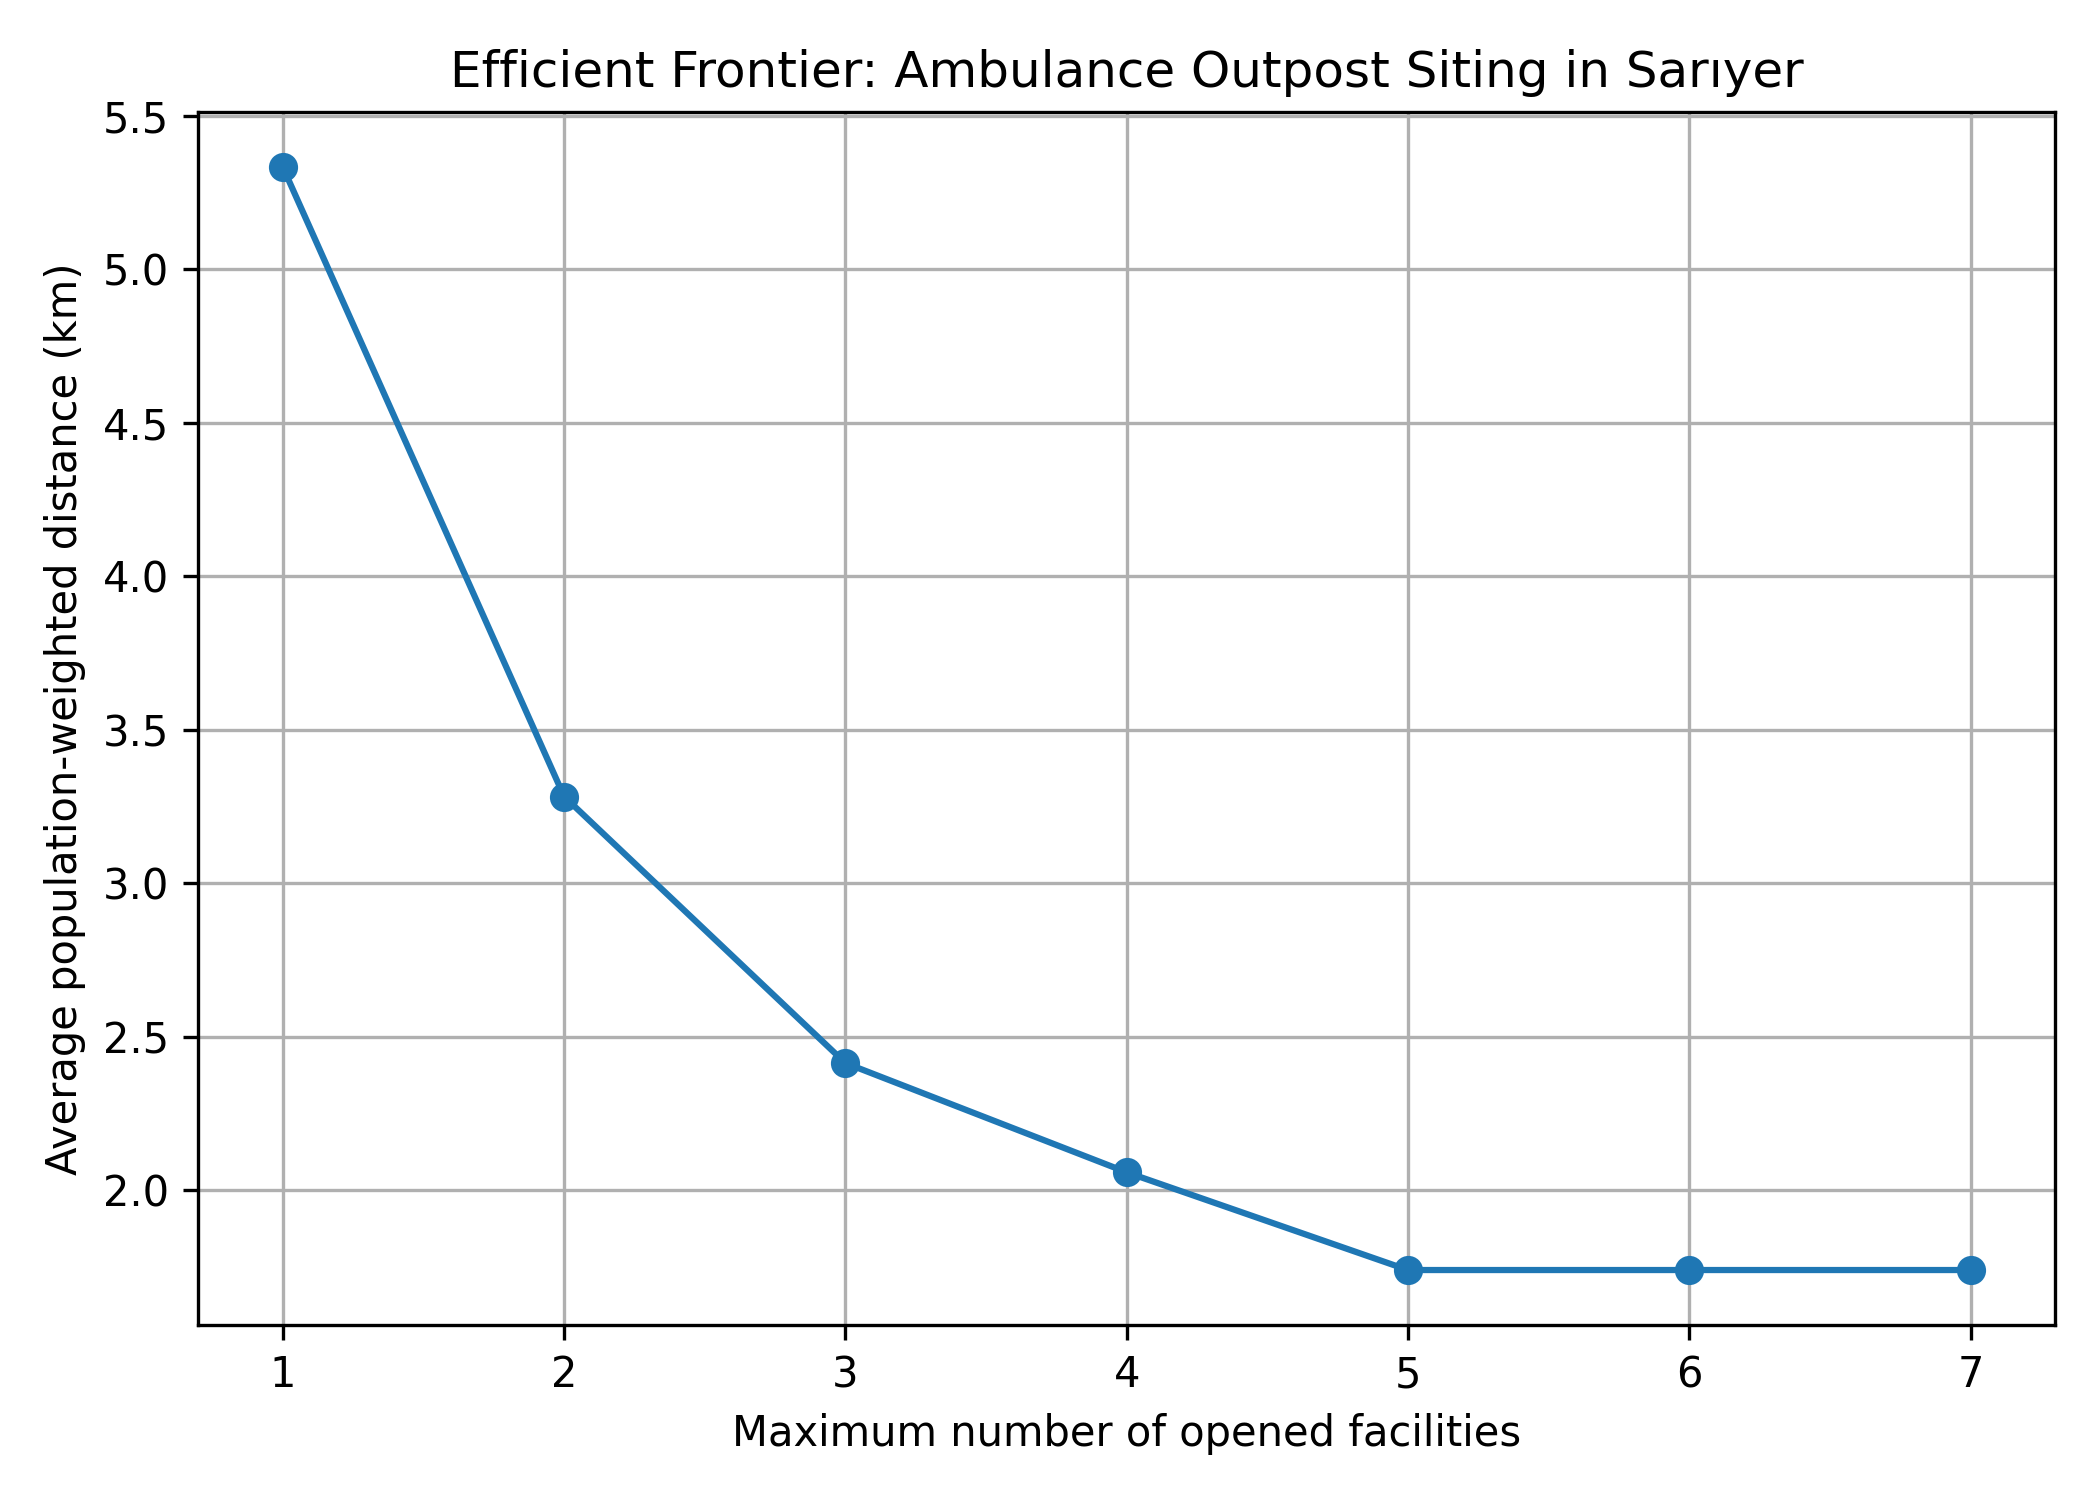
\includegraphics[width=0.85\textwidth]{../outputs/efficient_frontier_seed.png}
\end{frame}

\begin{frame}{Recommended Solution}
\begin{itemize}
    \item Recommended number of outposts: 4.
    \item Opened facilities: F2, F3, F6, F7.
    \item Average weighted distance: approximately 2.06 km.
    \item Maximum assigned distance: approximately 3.6 km.
    \item This solution balances accessibility, equity, and implementation cost.
\end{itemize}
\end{frame}

\begin{frame}{Assignments}
\begin{tabular}{ll}
\hline
Neighborhood & Assigned Facility \\
\hline
Ayazaga & F3 \\
Zekeriyakoy & F7 \\
Resitpasa & F3 \\
Tarabya & F2 \\
Fatih Sultan Mehmet & F2 \\
Istinye & F2 \\
Yenikoy & F2 \\
Ferahevler & F2 \\
Maden & F6 \\
Merkez & F6 \\
\hline
\end{tabular}
\end{frame}

\begin{frame}{Limitations}
\begin{itemize}
    \item Population is only a proxy for EMS demand.
    \item Real ambulance demand would require incident-level call data.
    \item Traffic and time-of-day effects are not modeled.
    \item The seed matrix should be refreshed with live road-network distances if possible.
\end{itemize}
\end{frame}

\begin{frame}{Conclusion}
\begin{itemize}
    \item The model provides a reproducible district-scale planning framework.
    \item Four facilities appear sufficient under the seed instance.
    \item Equity metrics show whether any neighborhoods remain poorly served.
    \item The framework can be extended with real EMS demand and travel-time data.
\end{itemize}
\end{frame}

\end{document}